\question[3]
Gib für den abgebildeten Graphen die Implementierung in Python als Adjazenzmatrix an.
Die Knoten a,b,c,.. sind auf die Indizes 0,1,2,... abgebildet.

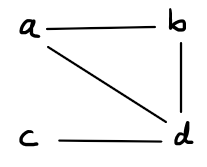
\includegraphics[height=3cm]{\pfad/Graphen/Aufgaben/adjazenzmatrix_04b/adjazenzmatrix_04b.png}
\begin{solutionbox}{4cm}
\begin{lstlisting}
G = [[0,1,0,1],
     [1,0,0,1],
     [0,0,0,1],
     [1,1,1,0]]
\end{lstlisting}
\end{solutionbox}
